\documentclass[12pt]{article}
\usepackage{geometry}
\usepackage{amssymb}
\usepackage[english]{babel}
\selectlanguage{english}
\usepackage[T1]{fontenc}
\usepackage[latin1]{inputenc}
\usepackage{fancyhdr}
\usepackage[]{algorithm2e}
\usepackage[usenames,dvipsnames]{xcolor}
\usepackage{array,tabularx,ragged2e,booktabs,caption}   % for \newcolumntype macro

\newcolumntype{L}{>{$}l<{$}}
\usepackage{multirow}
\usepackage{graphicx}
\usepackage{lastpage}

\usepackage{listings,lstautogobble}

%%
%% Julia definition (c) 2014 Jubobs
%%
\lstdefinelanguage{Julia}%
{morekeywords={abstract,break,case,catch,const,continue,do,else,elseif,%
		end,export,false,for,function,immutable,import,importall,if,in,%
		macro,module,otherwise,quote,return,switch,true,try,type,typealias,%
		using,while,Model,@constraint,@variable,@objective,solve},%
	sensitive=true,%
	alsoother={\$\\},%
	morecomment=[l]\#,%
	morecomment=[n]{\#=}{=\#},%
	morestring=[s]{"}{"},%
	morestring=[m]{'}{'},%
}[keywords,comments,strings]%

\lstset{%
	language         = Julia,
	basicstyle       = \ttfamily,
	keywordstyle     = \bfseries\color{blue},
	stringstyle      = \color{magenta},
	commentstyle     = \color{ForestGreen},
	showstringspaces = false,
	autogobble		 =true,
}

\geometry{
	a4paper,
	total={170mm,257mm},
	left=20mm,
	top=20mm,
}
\SetAlCapSkip{1em}
\title{%
		Homework 3 : Simulated Annealing and Genetic Algorithm \\
		\large University of Nantes \\
		Master 1 Optimization in operational research  \\
		Class of Metaheuristics \\
		Professor : Xavier Gandibleux	\\
		\vspace{4cm}
		\begin{figure}[h]
			\centering
			
\includegraphics[scale=0.20]{logo-un.png}
		\end{figure} 
	}
\author{
 \vspace{4cm}\\
	L\'eon Ferrari\\
	\small University of Nantes \\
	\small Master 1 Optimization in operational research\\
	Written with \LaTeX
 }
\graphicspath{ {images/} }
\pagestyle{fancy}
\rhead{Master 1 ORO - 2017 | L\'eon Ferrari }
\lfoot{University of Nantes | Metaheuristics}
\rfoot{Page \thepage /\pageref{LastPage}}


\begin{document}
	\maketitle
	\pagebreak
	\tableofcontents{}
	\pagebreak
	\section{Introduction to the Set Packing Problem}
	The Set Packing Problem with a finite size n of item and m of constraints.\\
	It can be define as follow, with :\\
	
	\begin{tabular}{LLLLL}
		Max \, Z & = &  \sum\limits_{i=1}^n x_{i} \, \times \, c_{i}  \\ 
		s.c. & \sum\limits_{i=1}^m\sum\limits_{j=1}^n x_{i,j}\, \times \, x_i & \leq &  1 \\
		x_{i} \in \{0,1\} \\
	\end{tabular}\\
	With : \\
	$$ x_i \quad where \left\{\begin{array}{ll}
	1 \quad if \, x_i \in solution. \\
	0 \quad otherwise\\
	\end{array}  \right\} \\$$ $$
	x_{i,j} \quad where \left\{\begin{array}{ll}
	1 \quad if \, x_{i,j} \in constraint \,i. \\
	0 \quad otherwise\\
	\end{array}  \right\} \\$$
	$ i \in [1,n], \quad j \in [1,m]$\\
	$x_i$ a variable of the solution.\\
	$c_i$ the cost of variable \textit{i}.\\
	$x_{i,j} $ an element of the constraint matrix.\\
	This type of problem can be illustrated in several ways, I will introduce you to some of them.
	\vspace{15pt} \\
	Illustration 1 :\\
	You are moving out of your apartment and you need to pack your different item.\\
	Obviously some of theses objects are more important for you or more expensive.\\
	But you do not have enough boxes so you will have to choose which one you will protect from a possible break.\\
	Here the coefficient of the objective value will be the value of the different items and the constraints will represent the boxes that you own.\\
	\vspace{5pt} \\
	Illustration 2 :\\
	You are a manager and you have to create a sport team for your company. In order to select them you send them to pass different test.\\ You also asked them with who they don't want be if they are in the sport team.\\
	Here the coefficient of the objective value will be the result of the test and the constraints will represent the people they don't want to be with.\\
	
	\subsection{JuMP modelisation for the set packing problem}
	 The modelling of the problem have been done with the language Julia and the package
	JuMP (Julia for mathematical programming). We used the GLPKSolverMIP , the GLPK
	solver for mixed-integer problem. Once the data describing the problem have been
	extract from the file, we can create a model with JuMP and send it to GLPK in order to solve it with the
	following instructions :\\
	\begin{lstlisting}[language=julia,caption={Configuration du demon SNMP}]
	#= This is a code modelling and solving a SPP problem with JuMP and GLPK) =#
	model  = Model(solver=GLPKSolverMIP())
	@variable( model,  x[1:n], Bin)
	@objective( model , Max, sum( Variables[j] * x[j] for j=1:n ) )
	@constraint( model , cte[i=1:m], sum(Constraints[i,j]* x[j] for j=1:n) 
	<= 1 )
	solve(model)
	\end{lstlisting}
	\subsection{Ten instances of the SPP}
	\begin{center}
		\begin{tabular}{|c|c|c|c|}
			\hline
			Problem Name & Number of Variables & Number of constraints & Best known value \\
			\hline
			100rnd0100.dat & 100 & 500 & 372\\
			\hline
			100rnd0200.dat & 100 & 500 & 34\\
			\hline
			100rnd0300.dat & 100 & 500 & 203\\
			\hline
			100rnd0400.dat & 100 & 500 & 16\\
			\hline
			100rnd0500.dat & 100 & 100 & 639\\
			\hline
			100rnd0600.dat & 100 & 100 & 64\\
			\hline
			100rnd0700.dat & 100 & 100 & 503\\
			\hline
			100rnd0800.dat & 100 & 100 & 39\\
			\hline
			100rnd0900.dat & 100 & 300 & 463\\
			\hline
			100rnd1000.dat & 100 & 300 & 40\\
			\hline
		\end{tabular}
	\end{center}
	
	
	

	\section{Genetic algorithm}
	
	During this second homework we had to choose an algorithm between ACO,GA and Simulated Annealing. I wanted to develop a genetic algorithm because of the many features that can be included and adjusted to fit the problem. For example there are many way of operating a crossover or a mutation. You can add some random individual into your population to diversify it and maybe avoid a local optimum etc.. All the tuning possible concerning the different crossover method, the probability of mutation etc. look interesting.
	
	I will now describe all the different component of my algorithm, beginning by the structure of an individual also called solution.
	
	\subsection{Data structure}
	\subsubsection{Problem data structure}
	To store the problem we will use two different type, a sparse matrix for the constraints and a vector for the coefficient of each variable.
	
	I tried to use the advantage of a sparse matrix, I noticed a significant improvement in time and complexity. The SPP is highly constrained problem but because of its structure where only a few variable are present in each constraint, that is why using a sparse matrix is useful. 
	\subsubsection{Chromosome data structure}A chromosome is  set of variables that define a solution. The population of a Genetic algorithm is composed of chromosome. 
	
	In my algorithm the chromosome is a data-structure composed of a vector, the solution, and an integer, the fitness value of the solution. The fitness value here is just the objective value of the problem.
	
	It's commonly noticed that the computation of the fitness value is the most expensive function in term of complexity. However the the structure of the set packing problem allow us to never really compute it because here we don't need the \textit{f(x)} being only a set of simple addition. So we just need to add or subtract the coefficient of a variable every time it is add or remove from the solution.
	\subsubsection{Population data structure}
	The population will be a vector of chromosome ordered by decreasing order of objective value.
	And every time a new "chromosome" will be created he will be added in this array in a way to keep the order and the last element of the array will be deleted.
	
	And if we keep the population ordered we do not need store the minimum or maximum fitness value of the population.
	\subsection{Building a feasible solution}
	\subsubsection{Greedy randomized adaptive search procedure (GRASP)}
	
	In a genetic algorithm you handle a population and apply different method on this group of solution in order to increase it. You try to mix solutions in order to build a better one. Because a GA use this strategies in order to crate new individual you want your base population to be diverse. And GRASP is perfectly adapted to build this kind of solution.
	
	It will allow us  to have a diverse, good and feasible population. 
	In order to build different good solution we will use the construction algorithm
	called GRASP from Mauricio G. C. Resende.
	The population for the genetic algorithm will be generated using GRASP.
	It is an easy to program and understand algorithm. The aim is too pick randomly the
	candidate which will be set to one through a random candidate list. 
	The major interest of this algorithm is the technique used create the random
	candidate list therefore a parameter, $ \alpha$, is used to built it. 
	$ \alpha$ is a coefficient used in the creation of the random candidate list, it
	will be used to compute a lower bound limit for the selection of the candidate
	variable. 
	
	Once we have compute the utility for each variables, in the case of the SPP problem
	the so called "utility" is :
	$$
	U_i =  \frac{c_i}{ \sum\limits_{j=1}^m x_{j,i}} 
	$$
	In the following steps \textit{Utility} will be considered as a Vector of size n
	containing the utility of each variable.
	The lower bound limit for the utility will be compute as follow : \\
	$$
	Limit = \min{(Utility)} + \alpha \times (\max{(Utility)} - \min{(Utility)})
	$$
	And now the construction algorithm :
	
	
	\vspace{10pt}
	
	\begin{algorithm}[H]
		\KwData{Alpha,V,C}
		\KwResult{Solution}
		\tcc{C the constraint matrix, V the variables cost}
		\tcc{Sort the array in decreasing order based on the second row }
		Utility = $\forall  v  \in V, U_v=\frac{Cost_v}{\sum\limits_{j=1}^m X_{j,v}} $\\
		\tcc{Sort by decreasing order}
		sort(Utility)\\
		\While{NotEmpty(RCL)}{
			Limit = Min(Utility) + Alpha * (Max(Utility)- Min(Utility))
			
			RCL = $ \emptyset$
			
			
			\For{i := 1 to N}{	
				\eIf{Utility[i] >= Limit}{
					RCL = add(RCL,i)
				}{
					break
				}
			}
			Candidate = RandomSelect(RCL)\\
			UpdateUtility(Utility)\\
			addToSolution(Solution,Candidate)\\
		}
		\Return Solution\\
		
		\caption{GRASP Construction}
	\end{algorithm}
\pagebreak
	\subsection{Parent selection}
	A roulette selection is used to find the parents that will produce the new element of the population. The roulette selection is simple it will randomly select two parents $X_1$ and $ X_2$ with the probability :
	$$
	p_x{_i} =  \frac{f_i(x) - f_{min}(x)}{ \sum\limits_{j=1}^n \left( f_{j}(x)- f_{min}(x) \right)} 
	$$
	In my algorithm four solution will be selected using the roulette selection and then a binary tournament will select the two future parents. A binary tournament is simple :
	
	\begin{algorithm}
		\KwData{$S_1,S_2,S_3,S_4$}
		\KwResult{$P_1,P_2$}
		\tcc{$S_i$ a solution $P_i$ a possible parent}
		\eIf{$S_1 > S_2$}{
			\eIf{$S_3 > S_4$}{
				$P_1=S_1$
				$P_2=S_3$
			}{
				$P_1=S_1$
				$P_2=S_4$
			}
			}{
			\eIf{$S_3 > S_4$}{
				$P_1=S_2$
				$P_2=S_3$
			}{
				$P_1=S_2$
				$P_2=S_4$
			}
		}
		return	$P_1$,$P_2$
		\caption{Binary tournament}
		\end{algorithm}
	\pagebreak
	\subsection{Crossover method}
	The crossover method is the most important part of the algorithm. It will allow us to create new individual/solution from the other by crossing them. Multiple methods exist to do a crossover between to solution using a binary mask for example
	Each crossover in my algorithm will produce two children combination of the parents. Because the method use for the crossover have a high chance to make the new solution infeasible we will have to repair the solution after.
	It is a called the two-fusion operator\footnote{A Genetic Algorithm-Based Heuristic for Solving the Weighted
		Maximum Independent Set and Some Equivalent Problems written by Mhand
		Hifi}
	Here is the crossover algorithm :
	\begin{enumerate}
		\item if  $P_{1,i} == P_{2,i}$
		\subitem set $C_{1,i} = C_{2,i} = P_{1,i} $
		\item else
		\subitem set randomly  k et k' ($k \neq k'$) a value in {1,2}
		\subitem set $ C_{1,j} = p _{k,j} $ with probability $p_k = f_k^f / f_k^f+f_{k'}^f$
		\subsubitem and $ C_{1,j} = p _{k',j} $ with probability $1-p_k$
		\subitem set $ C_{2,j} = p _{k',j} $ with probability $p_{k'} = f_{k'}^f / f_k^f+f_{k'}^f$
		\subsubitem and $ C_{2,j} = p _{k',j} $ with probability $1-p_{k'}$
	\end{enumerate}
	\begin{algorithm}
		\KwData{$P_1,P_2$}
		\KwResult{$C_1,C_2$}
		\tcc{$C_i$ a children, $P_i$ a parent}
		\For{i := 1 to N}{	
			\eIf{$P_{1,i} == P_{2,i}$}{
					
				$C_{1,i} = P_{1,i}$
				
				$C_{2,i} = P_{1,i}$
			}{
				$K_1$ = rand($1 \lor 2$)
				
				\eIf{$K_1 == 1$}
				{$k_2 = 2$}
				{$k_2 = 1$}
				$p_{k1} = f_{k1}(x) / f_{k1}(x) +f_{k2}(x)$
				
				$p_{k2} = f_{k2}(x) / f_{k1}(x) +f_{k2}(x)$
				
				\eIf{rand() $ < p_{k1}$}
				{$C_{1,i} = P_{k1,i}$}
				{$C_{1,i} = P_{k2,i}$}
				
				\eIf{rand() $ < p_{k2}$}
				{$C_{2,i} = P_{k2,i}$}
				{$C_{2,i} = P_{k1,i}$}
				
			}
		}
		return	$C_1$,$C_2$
		\caption{Crossover}
	\end{algorithm}
	\pagebreak
	\subsection{Mutation}
	\subsubsection{Repairing the solution}
	We explain that the crossover method may create infeasible solution. So we have to repair the solution, we use a simple method.
	Here is the algorithm :
	
	 \begin{algorithm}
	 	\KwData{$S_1,C$}
	 	\KwResult{$S_1$}
	 	\tcc{$S_i$ a solution,$C$ the constraints}
	 	\For{i := 1 to N}{	
	 		\If{$S_{1,i} == 1$}{
	 			\For{j := 1 to M}{
	 				\If{$C_{j,i} == 1$}{
	 					\For{$\forall S_{1,k} \in C_{j}$}{
	 						\If{$S_{1,k} \neq S_{1,i}$ and $S_{1,k} = 1$  }{
	 							$S_{1,k} = 0$
	 						}
	 					}	
 					}	
 				}
	 		}
	 	}
	 	return	$S_1$
	 	\caption{Repairing a solution}
	 \end{algorithm}
 	\subsection{Improving a solution}
 	It's a greedy algorithm of descent, where he go throught the variable and if a variable  is free he set it to one.
 	\subsection{Parameters \& stop conditions}
 	Our algorithm don't have yet a mutation method because the crossover imply to repair and do LS on the solution, so it implicitly execute a mutation. 
 	
 	But we have a probability of crossover of 30\%, knowing that two children are produced at each crossover it is a really high probability of crossover.
 	
 	And our algorithm have two stop condition, when the number of generation is over the limit or when the population converge in value, we consider that an algorithm converge in value when $Stop_i$ is below 0.01 :
 	$$
 	Stop =  \frac{f_{max}(x) - f_{min}(x)}{f_{avg}(x)} 
 	$$
 	I set the number of generation to 30 but the algorithm will mainly stop because of the stop condition than because he reached the 30th generation. He will only reach the 30th generation for big sized problem.
 	\pagebreak
	\section{Results and performances}
	In this chapter we will compare the result obtained by our previous "heuristics" and the genetic algorithm. I will also introduce the environment the algorithm is running on.
	\subsection{System and environment}
	We solved the problem on the following system :
	\begin{center}
		\begin{tabular}{|c|c|}
			\hline
			OS & Centos 7 64 bits \\
			\hline
			Processor & i7 4720HQ \\
			\hline
			CPU Freq & 2.6GHz \\
			\hline
			Physical Core CPU & 4 \\
			\hline
			RAM & 8GB \\
			\hline
			Julia & Version 0.6.0 \\
			\hline
			Solver & GLPK\\
			\hline
		\end{tabular}
	\end{center}

	Below the heuristic construction go with the LS, the generation of the population is included in the time of the GA.
	We obtained the following result :
	\begin{center}
		\begin{tabular}{|c|c|c|c|c|c|c|}
			\hline
			Problem  &\multicolumn{2}{|c|}{Grasp construction} & \multicolumn{2}{|c|}{Local search}& \multicolumn{2}{|c|}{Genetic algorithm}\\
			\hline
			Data  &  $\tilde{Z_{avg}}$ & Time(s) & $\tilde{Z_{avg}}$ & Time(s)& $\tilde{Z_{avg}}$ & Time(s) \\
			\hline
			100rnd0100  & 338.755 & 0.0001 &  352.01 & 0.05 & 369.12 & 0.18\\
			\hline
			100rnd0200  & 29.675  &  0.0001 &  33.985 & 0.06 & 32.0 & 0.1\\
			\hline
			100rnd0300  & 181.265   & 0.0555 & 185.81 & 0.06 &197.84 & 0.18\\
			\hline
			100rnd0400 & 13.295    & 0.0606 & 15.31 & 0.07 &15.16&0.1\\
			\hline
			
			100rnd0500  & 617.24     & 0.0001 & 621.435 & 0.02 & 631.48 & 0.04\\
			\hline
			
			100rnd0600  & 61.5     & 0.0235 & 64 & 0.0067 & 64.0 & 0.04\\
			\hline
			
			100rnd0700  & 491.715 & 0.0001025 & 497.7 & 0.02
			& 495.3 & 0.03\\
			\hline
			
			100rnd0800  & 35.99 & 0.0437 &38.32 & 0.02 &37.76& 0.03\\
			\hline
			
			100rnd0900  & 431.85     & 0.0001 & 446.84 & 0.04 &453.98&0.07\\
			\hline
			
			100rnd1000 & 36.17     & 0.0001 & 39.525 & 0.04 &38.5&0.074\\
			\hline
		\end{tabular}
	\end{center}
	Here we can observe that the genetic algorithm is slower but find an higher average value in general.

	We will compare now two algorithm the genetic algorithm and an algorithm based on multiple grasp construction where we apply a simulated annealing.
	
	We will compare the two algorithm on these various sized problem :
	\begin{center}
		\begin{tabular}{|c|c|c|c|}
			\hline
			Problem & N & M & Best Z \\
			\hline
			\textit{100rnd0100.dat} & 100 & 500 & 372 \\
			\hline
			\textit{200rnd0300.dat} & 200 & 1000 & 731 \\ 
			\hline
			\textit{500rnd0100.dat} & 500 & 2500 & 323  \\
			\hline
			\textit{1000rnd0300.dat} & 1000 & 5000 & 661 \\
			\hline
		\end{tabular}
	\end{center}
		
	Here are the different parameters used :
	\begin{enumerate}
		\item GRASP construction
		\subitem $ \alpha = [0.5,0.6,0.75,0.90]$
		\subitem $ p_{\alpha} = [0.25,0.25,0.25,0.25]$
		\item Genetic algorithm
		\subitem Size of the population : 100.
		\subitem Generation : 30.
		\subitem Probability of crossover : 30\%.
		\item Simulated annealing
		\subitem 20 construction
		\subitem Cooling coefficient : 0.95
		\subitem Init temperature : 1000
		\subitem Step size : 100
		\subitem Stop temperature : 1.0
	\end{enumerate}
	For the parameter of population, I think It should be sized according to the problem but I don't know how I correctly tune it. For example we can have a bigger population for small sized (100 or 200 variables) problem as it take a small amount of time. 
	
	But for bigger we could may be reduce it to be faster however it is not really logical as "more" solution will exist so a bigger population will be needed to express the diversity of possible solution.
	
	So for the problem \textit{500rnd0100.dat} and \textit{1000rnd0300.dat} we will run the genetic algorithm with different population size and stop conditions.
	
	\begin{center}
			\begin{tabular}{|c|c|c|c|c|}
				\hline
				Problem &\multicolumn{4}{|c|}{Simulated annealing} \\
				\hline
				& $\tilde{Z_{min }}$ & $\tilde{Z_{avg}}$ & $\tilde{Z_{max}}$&Time(s) \\ 
				\hline
				100rnd0100.dat & 336 & 349.5 & 363 & 0.64  \\
				\hline
				200rnd0300.dat& 645 & 685.2 & 708  & 1.01  \\
				\hline
				500rnd0100.dat& 239 & 269.75 & 288  & 6.18 \\
				\hline
				1000rnd0300.dat& 457 & 524.15 & 573 &  12.38 \\
				\hline
			\end{tabular}
	\end{center}
	\begin{center}
		\begin{tabular}{|c|c|c|c|c|c|c|c|c|}
			\hline
			Problem & \multicolumn{8}{|c|}{Genetic algorithm} \\
			\hline
			 & \multicolumn{2}{|c|}{Parameter} & \multicolumn{3}{|c|}{f(x)} & \multicolumn{3}{|c|}{Time}   \\
			\hline
			& Population & Limit  & $\tilde{Z_{min }}$ & $\tilde{Z_{avg}}$ & $\tilde{Z_{max}}$ & Min & Avg & Max\\
			\hline
			100rnd0100.dat & 50  & 0.01 
			& 365 & 370.15 & 372 & 0.14 & 0.2 & 0.32 \\
			\hline
			100rnd0100.dat & 50  & 0.05
			& 361 & 367.65 & 372 &0.08 &0.12 & 0.24 \\
			\hline
			100rnd0100.dat & 100 & 0.01 
			& 367 & 371.55 & 372 & 0.22& 0.37 & 0.45 \\
			\hline
			100rnd0100.dat & 100 & 0.05 
			& 365 & 367.15 & 372 & 0.18 &  0.23 & 0.31\\
			\hline
			200rnd0300.dat & 50  & 0.01 
			&  696& 706 & 712 & 0.58 &0.73& 0.98 \\
			\hline
			200rnd0300.dat & 50  & 0.05
			& 687 & 697.6 & 708 & 0.25 & 0.32 & 0.41
			\\
			\hline
			200rnd0300.dat & 100 & 0.01
			& 696 & 707.85 & 715 & 1.21 &1.49 & 2.16\\
			\hline
			200rnd0300.dat & 100 & 0.05
			& 687 & 697.45 & 709 & 0.46 & 0.61 & 0.89
			\\
			\hline
			500rnd0100.dat & 50  & 0.01 &
			289 & 307.75 & 319 & 15.1 & 21.13 & 29.5
			\\
			\hline
			500rnd0100.dat & 50  & 0.05
			& 289& 298.5& 311& 7.16& 14.41 & 25.01
			\\
			\hline
			500rnd0100.dat & 100 & 0.01
			& 299 & 309.3 & 320 & 34.5 & 48.27 & 65.5
			\\
			\hline
			500rnd0100.dat & 100 & 0.05 & 289 & 304.85 & 319 & 17 & 38.83 & 59.03
			\\
			\hline
			1000rnd0300.dat & 50  & 0.01 & 568 & 589.4 & 634 & 68.06 & 110.04 & 141.96
			\\
			\hline
			1000rnd0300.dat & 50  & 0.05 & 561 & 578.75 & 603 & 56 & 76.73 & 108 
			\\
			\hline
			1000rnd0300.dat & 100 & 0.01 & 575 & 596 &611 & 194& 276 & 329
			\\
			\hline
			1000rnd0300.dat & 100 & 0.05 & 567 & 593.6 & 628 & 179.2 & 230.5 & 322.54 
			\\
			\hline
		\end{tabular}
	\end{center}
	We can see that the GA has generally better result and if it is fast for small problem it is long for medium/big sized problem. 
	
	We can see that increasing the value of the limit or lowering the size of the population drastically change the execution time at the cost of the global score of the popullation. 
	
	But we are here interested only in the best solution found so far and  not the "global value" of the population. 
	If the population converging on a value can be a stop condition it does imply that all the population have the same value.
	
	Lowering the value of the limit could be done for any problem even if it could lead to be blocked in a local optimum.
	
	The couple GRASP + CS can found a solution in a really short amount of time compare to the GA but it is solution of lower quality. Also maybe if we modified some parameter to let it run as long as the GA it might found a better solution.
	
	I have tried, and it didn't, the solution are always worst or equal to the average solution of the GA.
	
	I collected the time spend in each function for the problem \textit{500rnd0100.dat} :
	\begin{center}
		\begin{tabular}{|c|c|c|}
			Function Name & Role & Time \\
			BinaryTournament & Select Parents & 0.000010 \\
			CrossoverMethod & Create new childrens & 0.000049\\
			RepairSolution & Repair a children & 0.017485 \\
			AugmentIndividual & Improve a solution by a LS & 0.159890 \\
			InsertAndReplaces & Insert child in ordered array & 0.000009 \\
		\end{tabular}
	\end{center}
	AugmentIndividual and RepairSolution are the most time expensive function and they executed for every new children created.
	The only improvement I found was to test if a children is equal to one of his parents, if it is none of this two function will be executed (Because the children is already a feasible and not improvable solution).
	
	I should maybe change the LS for a random mutation, it would have required more generation making the algorithm slower. It's a part that, if I had the time I would have develop and code.
	\pagebreak
	\subsection{Interpreting the results}
	Here are some plot of my GA :
	\begin{center}
		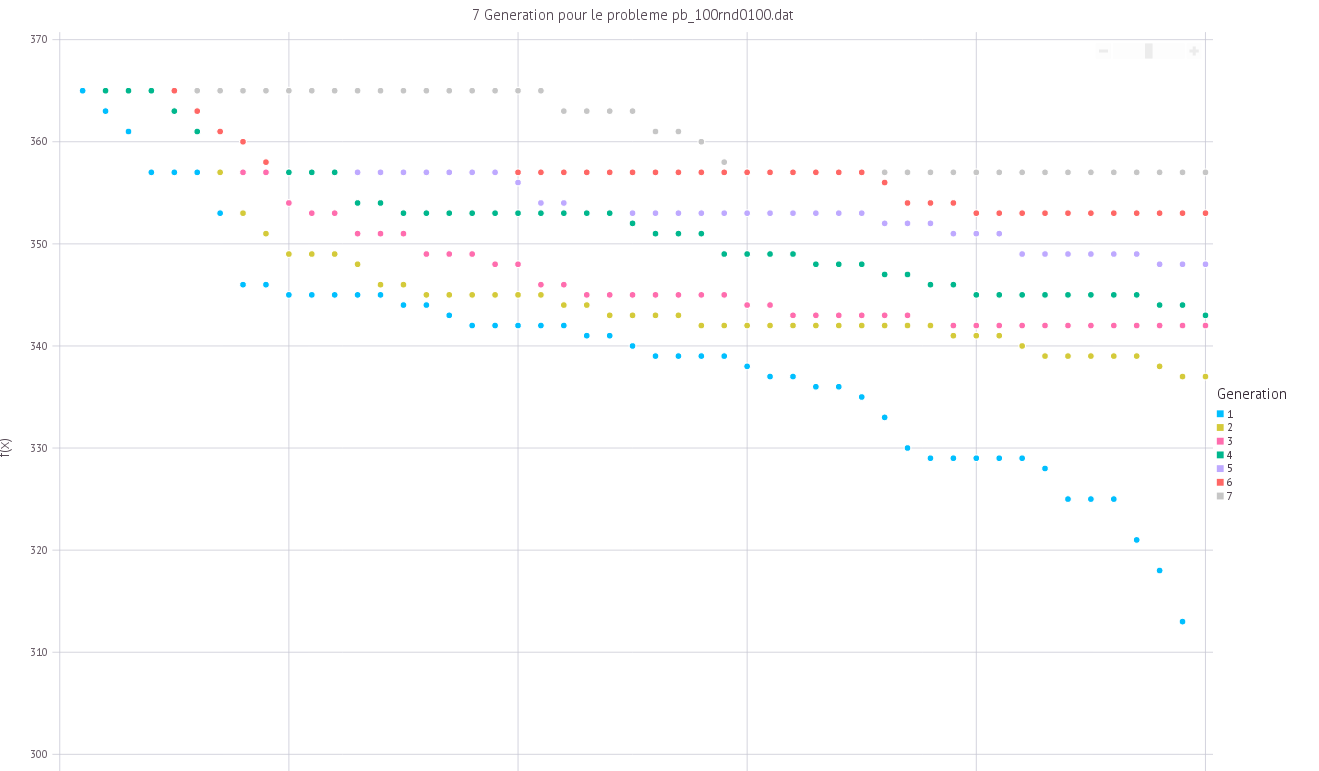
\includegraphics[scale=0.5]{100rnd0100.png}
		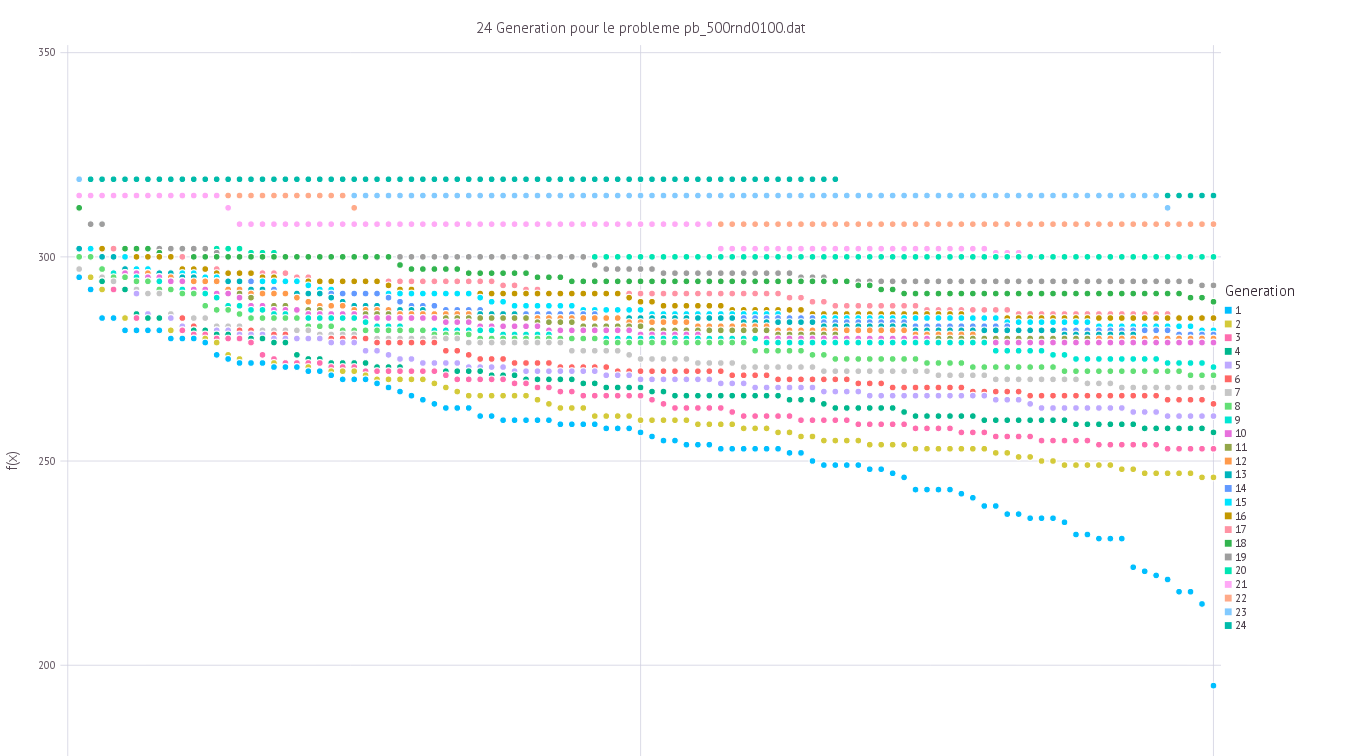
\includegraphics[scale=0.5]{500rnd0101.png}
		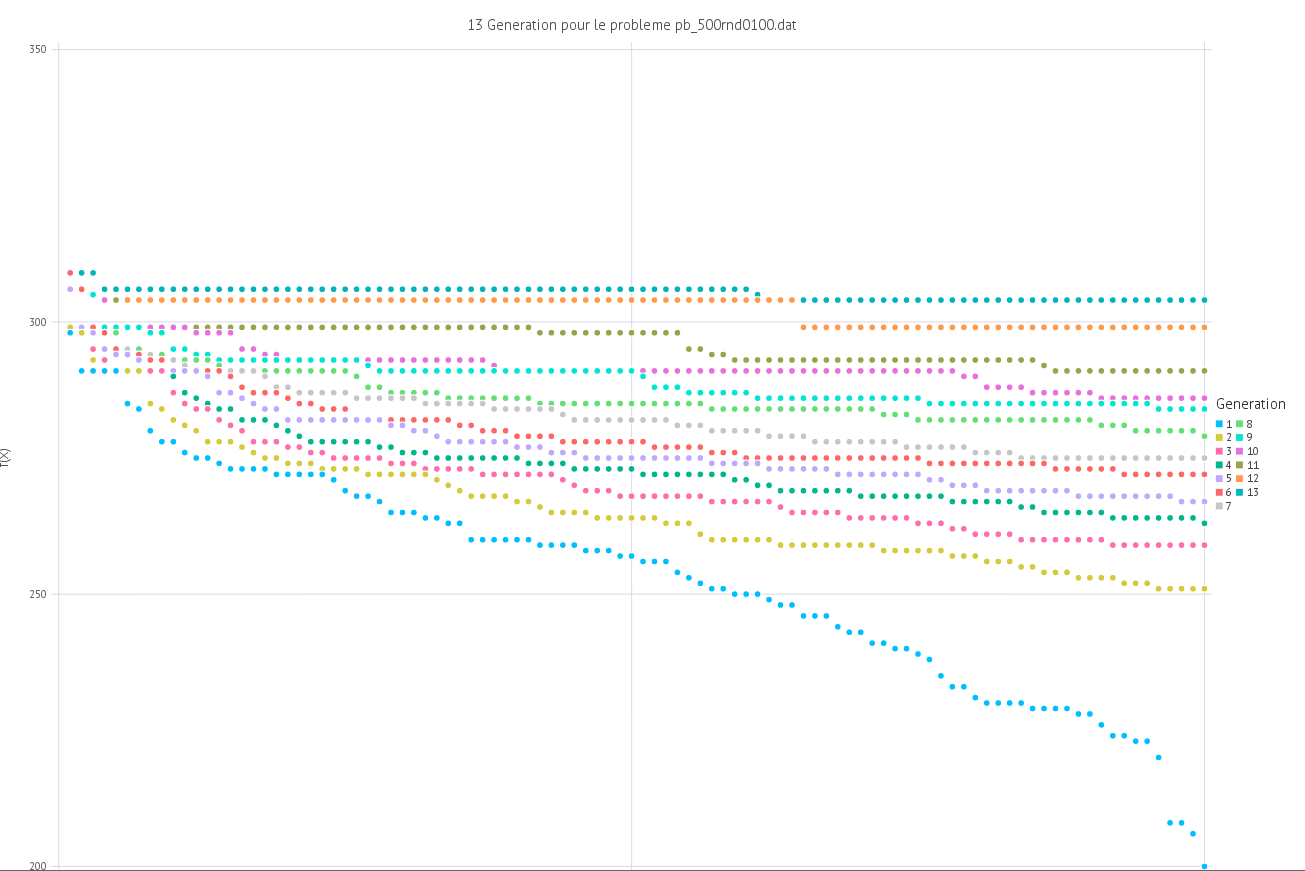
\includegraphics[scale=0.5]{500rnd0102.png}
		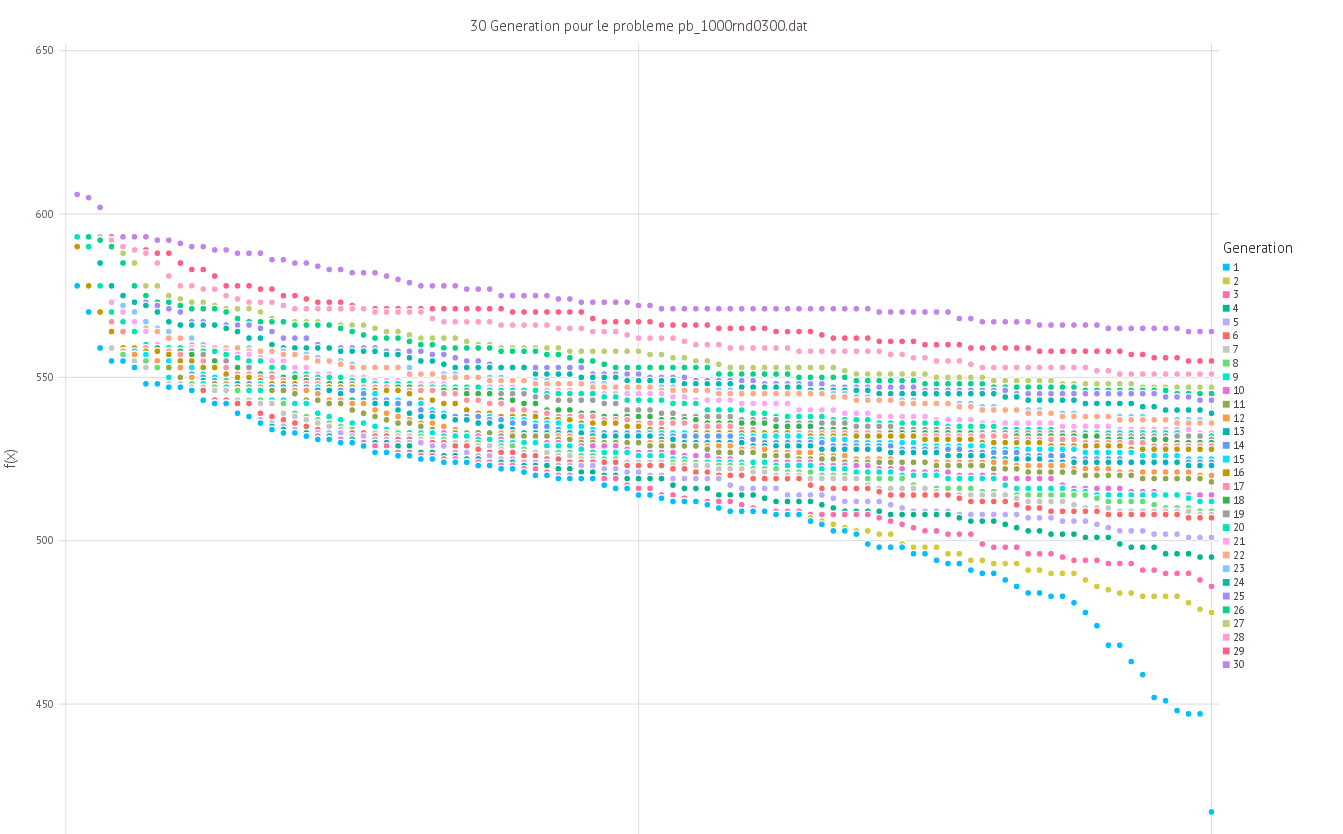
\includegraphics[scale=0.5]{1000rnd0300.png}
	\end{center}
	The decreasing f(x) is coming from the fact that the individual are sort in decreasing order by there objective value.
	
	We can see in the second plot that the generation 24 have nearly all here individual at the same level. They probably converge on the same solution.
	
	As generation increase we see the worst value disappear and the diversity of our population decreasing.
	
	We can also noticed on the 3rd and 4th plot that some individual are over the "convergence" bar. The GA may have stopped too soon because it could have used this individual to maybe reach a better solution.
	
	\section{Conclusion}
	
	This last homework was interesting thanks to the multiple strategy you could use in a GA and the freedom it offer. I would have like to introduce some other function, like the random add of a new individual or a real mutation. But it didn't looked necessary on the kind of problem we were running our algorithm.
	
	Different problem allowing more complex strategy could be fun and may be learn some tricks that are applicable to some kind of problem could be interesting. 
	
	I've tried to implement and use sparse matrix in the GA because with my previous work it was too slow. I did it successfully but there is still the construction algorithm based on GRASP that use my previous work. I began to work on a construction algorithm made specially for the GA and independent of all my previous work but I didn't had the time to finish it.
	
	I've also been using Julia embedded function as much as possible to make the program faster, but it happen once that a Julia function was slower than my code(Because of a stop condition).
	
	I was afraid to use VNS or Path-Relinking as a LS because it is easy, fast and does not need tons of new data to be used.However as it could have lowered the diversity of the population I decided to not.
	
	I don't know if it was possible to just use a crossover and mutation in my GA, as it is a highly constraint problem it looked difficult to rely only on these two method to get a good solution.
	
\end{document}